\begin{figure}[ht]
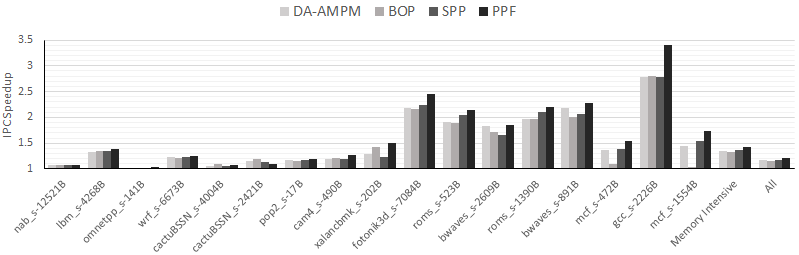
\includegraphics[width=\columnwidth]{SPEC2017}
\caption{SPEC CPU 2017 Single-Core IPC Speedup}
\label{Fig:SPEC2017_1core}
\end{figure}

\section{Results}
\label{Results}

This section discusses the results obtained from running PPF in terms
of speedup and prefetch cache, for the SPEC CPU 2017 benchmarks.
First, we present the results for single-threaded workloads then for
multi-core workloads.

\subsection{Single-core Results}
\label{Results-Single}

Figure~\ref{Fig:SPEC2017_1core} shows the single core speedup obtained
by BOP, DA-AMPM, SPP and PPF for each of the individual SPEC CPU 2017
applications, followed by the geomean of the memory intensive subset
and finally the geomean across the full suite.  All the results have
been normalized to the baseline of no prefetching.

PPF yields a geometric mean speedup of \textbf{26.95\%} over the
baseline.  This is equivalent to \textbf{4.63\%} over DA-AMPM,
\textbf{4.61\%} over BOP and \textbf{3.78\%} over SPP.  Out of the 20
SPEC CPU 2017 applications, PPF nearly matches or
outperforms all the other prefetchers on 19 applications.  
Benchmarks {\tt 603.bwaves\_s}, {\tt 605.mcf\_s}, {\tt{623.xalancbmk}\_s} 
and {\tt 649. fotonik3d\_s} benefit the most from PPF, with the 
speedup over SPP ranging from \textbf{10\% to 25\%}.

One interesting
case here is {\tt 623.xalancbmk}.  Despite SPP under performing on that
application, PPF manages to considerably outperform all prefetchers.
Since this benchmark has varying prefetch deltas, SPP's conservative
throttling mechanism catches that and quickly halts prefetching at an
average depth of 2.1.  On the other hand, PPF's more efficient
accuracy check enables it to prefetch up to a lookahead depth of
3.3. Doing this, PPF suggests 1.61 times more total prefetches and
2.53 times more useful prefetches than SPP.

The only benchmark where PPF fails to match the improvement offered by
any other prefetcher is {\tt 607.cactuBSSN\_s}. Based on our observation
of prefetching behavior, we gather that BOP's aggressive and localized
nature fits this workload very well; as opposed to SPPs lookahead
nature.  As a result, SPP, and hence PPF, underperform on this
benchmark.

On the full SPEC CPU 2017 suite, PPF improves the geometric mean IPC
of the baseline by \textbf{15.24\%}, which is \textbf{2.27\%} better
than the next best prefetcher -- SPP. {For PPF, the average 
lookahead depth over the full benchmark is 3.97, while it is 3.28 for just 
SPP. It is evident that on average for SPP, our scheme allows the 
prefetcher to speculate 21\% deeper.}

\begin{figure}[ht]
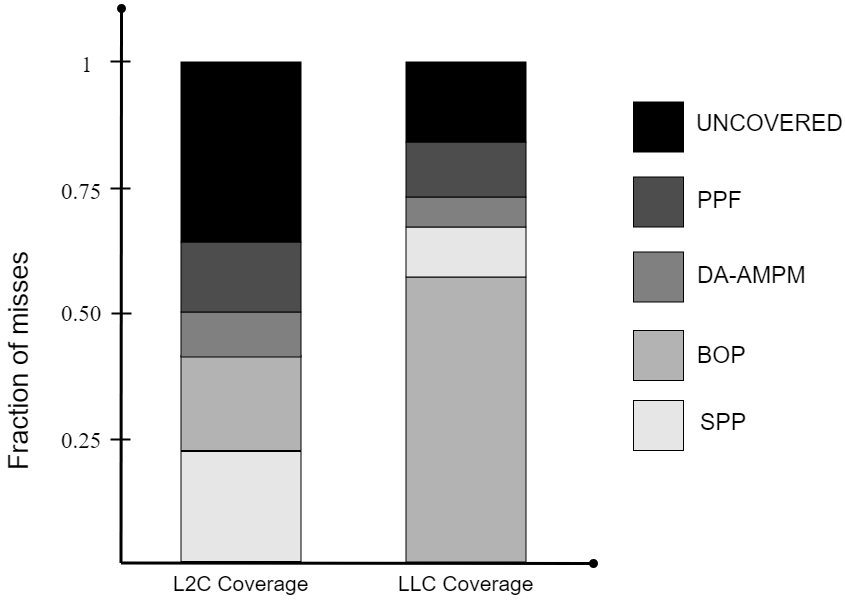
\includegraphics[width=\columnwidth]{Coverage}
\caption{Fraction of Cache Misses Covered}
\label{Fig:Coverage}
\end{figure}
%

\noindent \textbf{Coverage:} Prefetcher coverage is defined as the
ratio of the number of misses avoided through prefetching over the
number of misses with no prefetching.  Figure~\ref{Fig:Coverage} shows
the fraction of misses in the L2 and LLC avoided by the various
prefetchers.  PPF has the highest coverage of all the prefetchers
simulated.  On the SPEC CPU 2017 benchmarks, PPF reduces misses by
\textbf{75.5\%} and \textbf{86.9\%} in the L2 and LLC
respectively. For the same benchmarks, the next best prefetcher,
DA-AMPM, covers \textbf{54.3\%} and \textbf{78.5\%} of the misses
respectively.

This superior coverage of PPF can be attributed to aggressive
re-tuning of the underlying SPP, enabled by the Perceptron Filter
making sure the high coverage does not lead to increased cache
pollution.

\begin{figure}[ht]
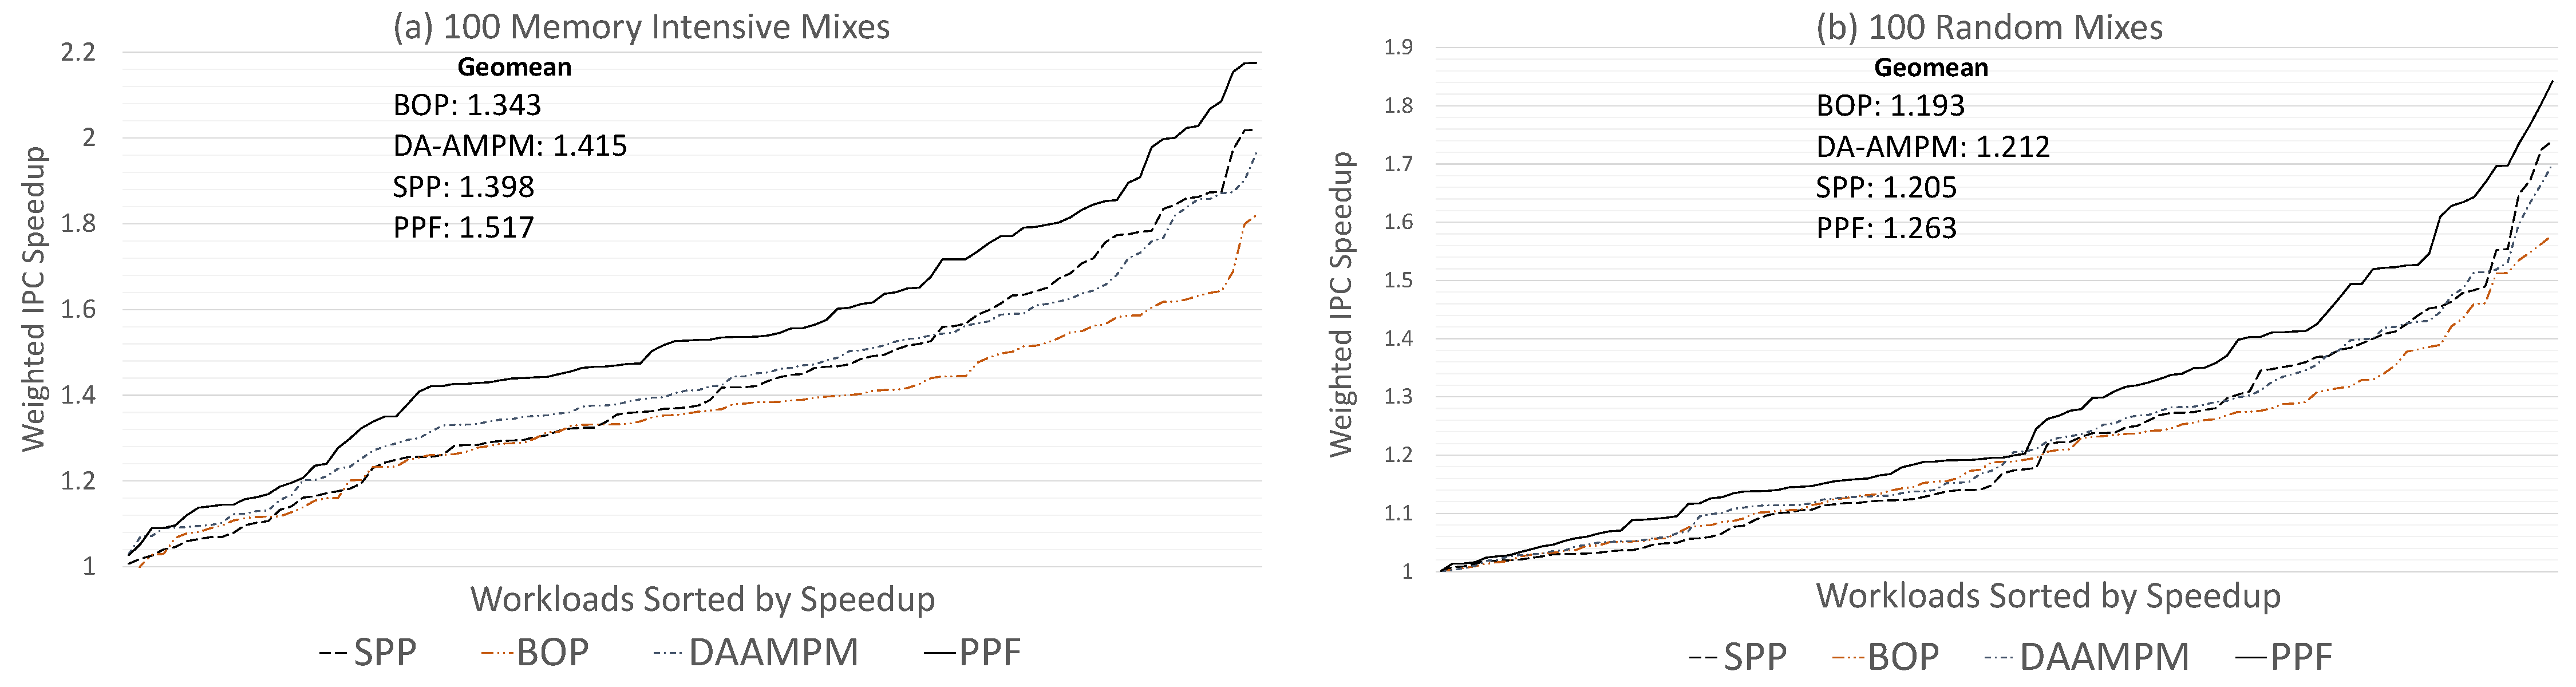
\includegraphics[width=2.75in]{4Core_SPEC2017}
\caption{Speedup for 4-core SPEC CPU 2017}
\label{Fig:4Core_SPEC2017}
\end{figure}

\subsection{Multi-core Results}
\label{Results-Multi}
\noindent In this section, we demonstrate the improvement achieved by PPF for a
mix of multi-programmed workloads.
\newline
\newline
\noindent \textbf{4-Core:} Figure~\ref{Fig:4Core_SPEC2017}
shows a comparison of speedups obtained on 4-core mixes of a memory
intensive subset of SPEC CPU 2017. We plot all 4 prefetchers, normalized
to the baseline. The workloads have been sorted in increasing order of
the speedup. PPF offers a speedup of \textbf{51.2\%} on these traces,
an improvement of \textbf{11.4\%} over the underlying SPP,
\textbf{9.7\%} over the next DA-AMPM, and \textbf{16.9\%} over BOP.
On a different set of fully random SPEC CPU 2017 4-core mixes (not
illustrated for space reasons), PPF provides an IPC speedup of
\textbf{26.07}\% over the
baseline, which is an improvement of \textbf{5.6}\% over SPP.
%
\begin{figure}[ht]
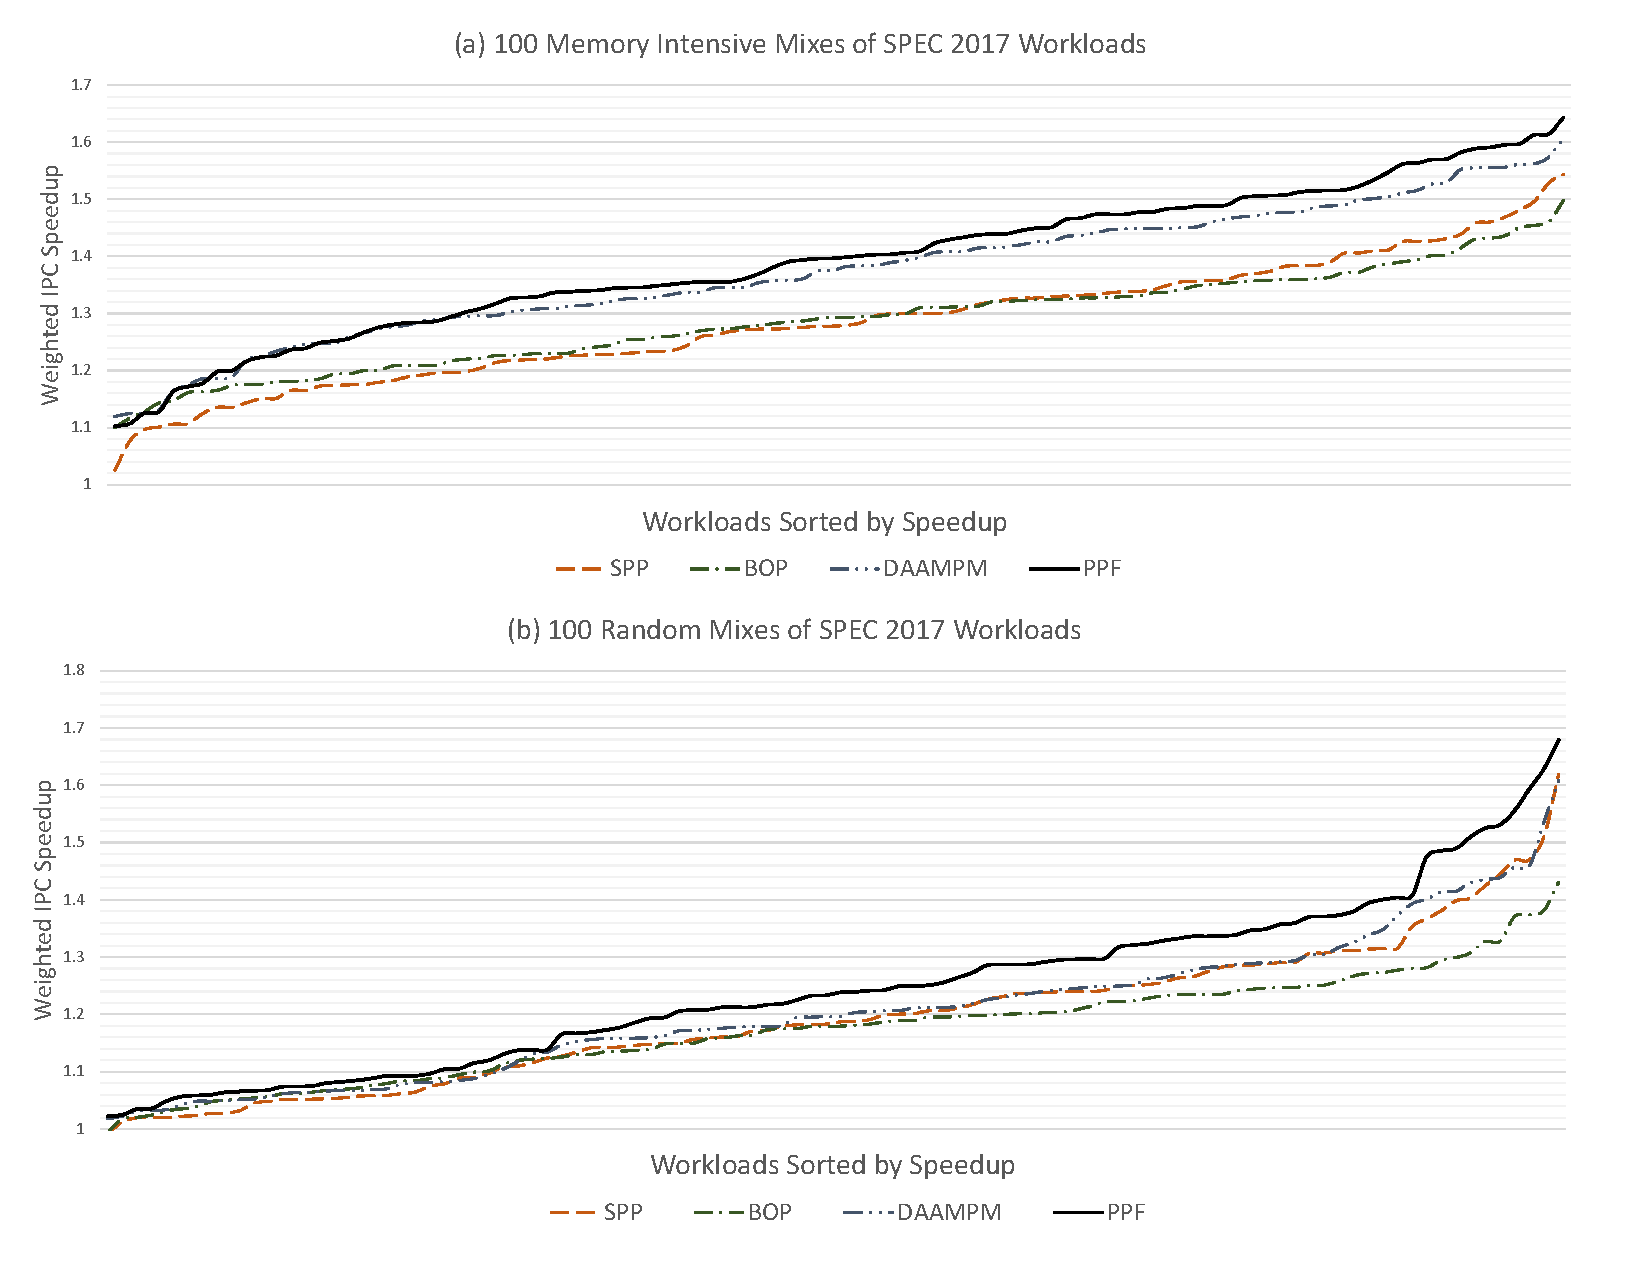
\includegraphics[width=2.75in]{8Core_SPEC2017}
\caption{Speedup for 8-core SPEC CPU 2017}
\label{Fig:8Core_SPEC2017}
\end{figure}
%
\newline
\newline
\noindent \textbf{8-Core:} The sorted comparison of speedups on the
memory intensive 8-core mixes is shown in
Figure~\ref{Fig:8Core_SPEC2017}.  PPF improves baseline performance by
\textbf{37.6\%}, an improvement of \textbf{9.65\%} over SPP. For a
random set of SPEC CPU 2017 mixes (not illustrated for space reasons),
PPF improves performance by \textbf{23.4\%} over the baseline,
corresponding to \textbf{4.6\%} over SPP. This increased improvement
achieved by PPF over the {underlying prefetcher, SPP,} 
in a multi-core environment is expected as PPF is a very accurate filter. 
Thus, it eliminates useless prefetches before they can cause pollution in the 
shared LLC. BOP offers a better improvement than SPP for the memory intensive
mixes. This superiority can be attributed to BOP's inherent aggressive
nature. DA-AMPM is also ahead of SPP in both the mixes. Interestingly,
in all these cases, PPF consistently outperforms the best performing
prefetcher.

\subsection{Additional Memory Constraints}
\label{Results-AdditionalMem}

We also model PPF with reduced LLC and with low bandwidth constraints,
respectively (not illustrated for space reasons).  Benchmark {\tt
  605.mcf\_s} in low bandwidth conditions is prefetch averse. In
general, any prefetcher yields a negative speedup on that trace. On
{\tt 654.roms\_s} and {\tt 607.cactuBSSN\_s}, PPF is unable to match
the performance achieved by the best prefetcher. On the other hand,
PPF outperforms all the other prefetchers on {\tt 623.xalancbmk\_s}
and {\tt 638.imagick\_s} benchmarks.  Overall, PPF provides a greater
improvement under small LLC condition and matches the best prefetcher,
BOP, under low DRAM bandwidth conditions.

\begin{figure}[ht]
\begin{adjustwidth}{-0.4cm}{}
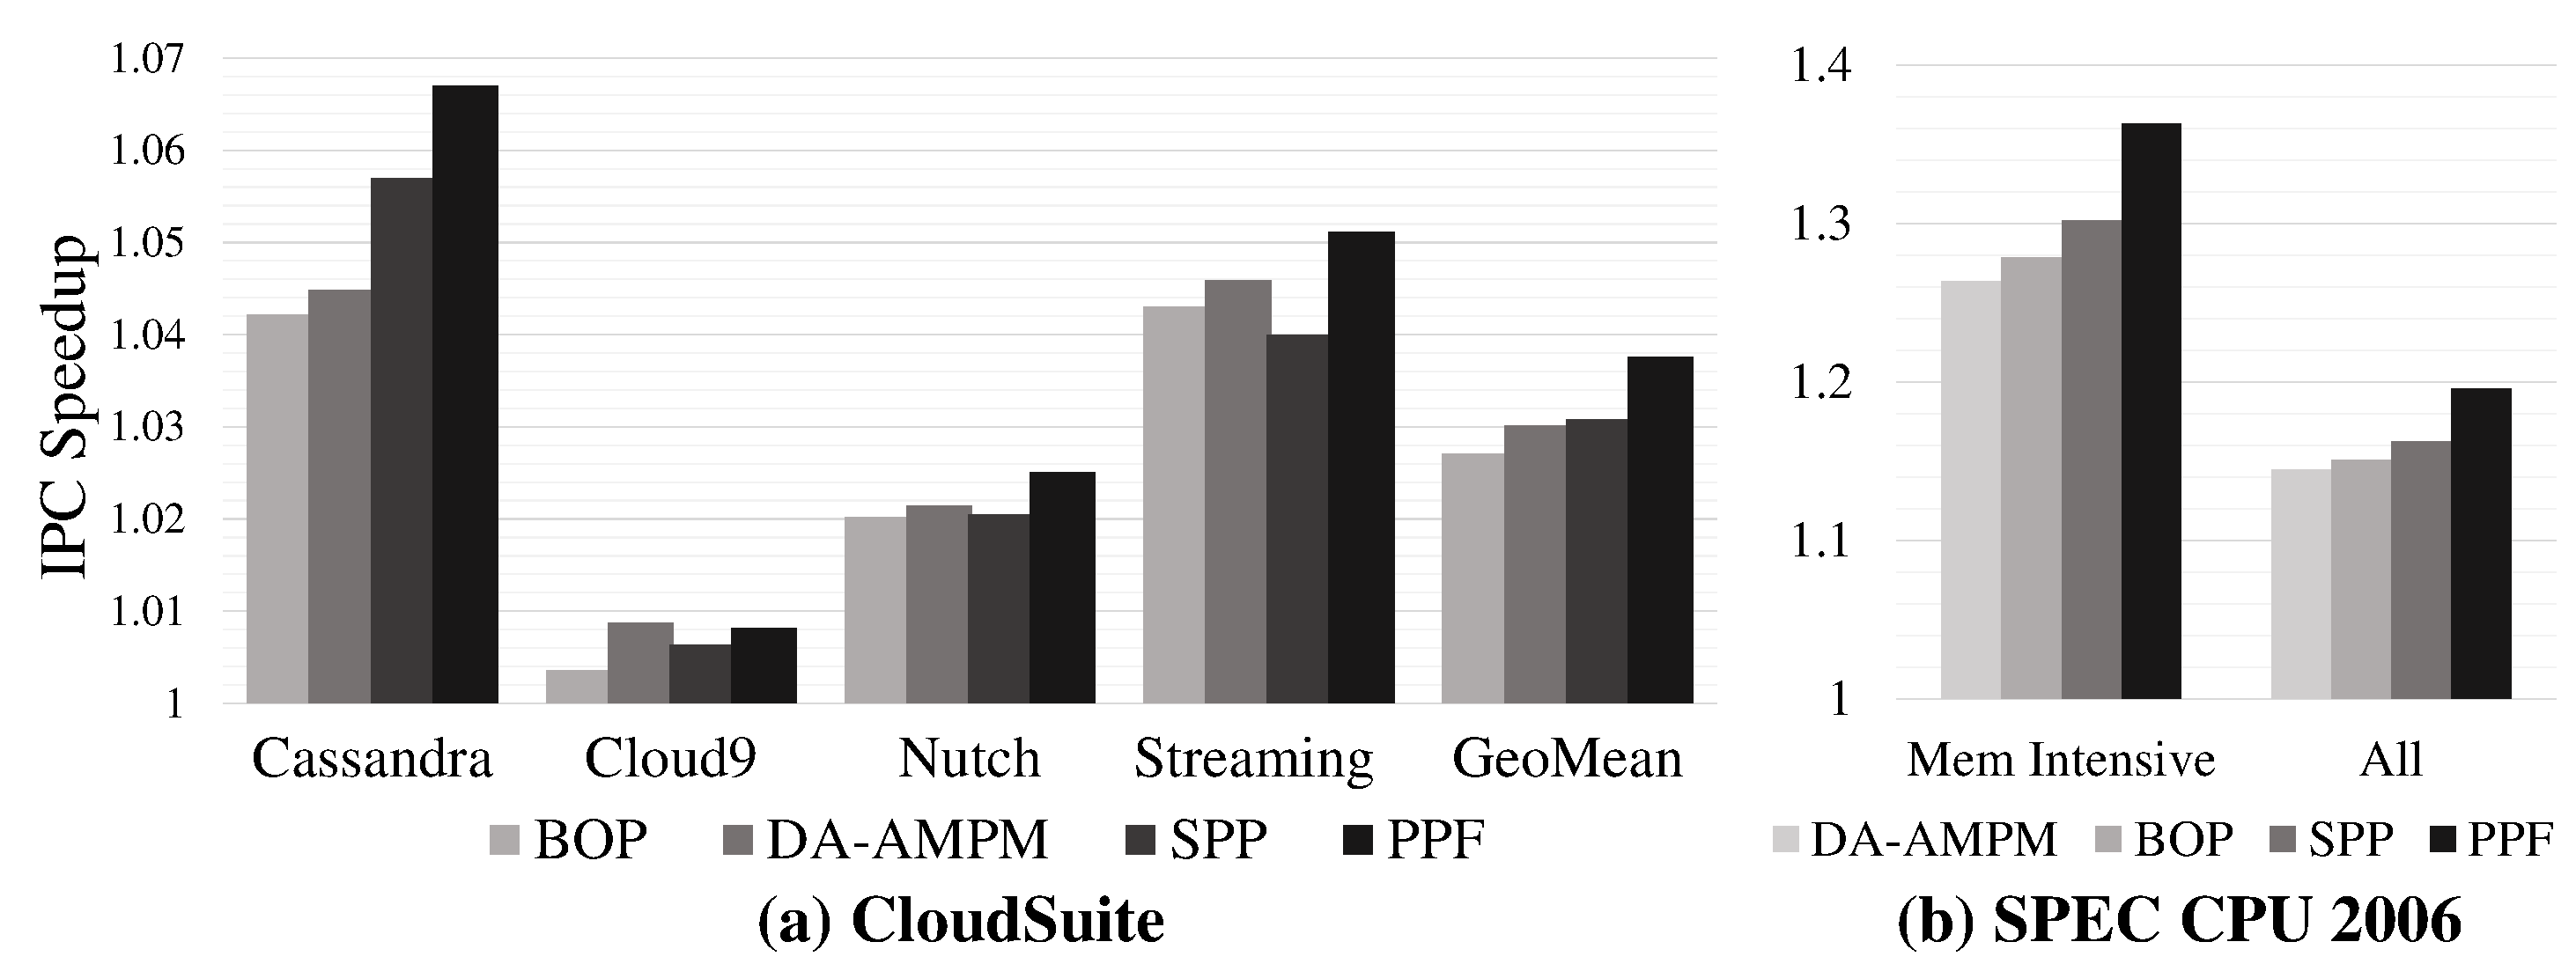
\includegraphics[width=1.1\columnwidth]{CrossVal}
\caption{IPC Speedup for Unseen Workloads}
\label{Fig:CrossVal}
\end{adjustwidth}
\end{figure}

\subsection{Cross Validation}
\label{Results-CrossVal}

Figure~\ref{Fig:CrossVal}(a) shows the performance benefit comparison
of all the prefetch schemes on 4 different applications in the
CloudSuite benchmark.  In general, these applications are prefetch
agnostic.  Even so, PPF manages a \textbf{3.78\%} improvement over no
prefetching, putting it ahead of the next best prefetcher, SPP, which
provides a 3.08\% speedup.

Figure~\ref{Fig:CrossVal}(b) shows the speed-up achieved on the memory
intensive subset and the full SPEC CPU 2006 suite for a
single-processor machine.  PPF provides a speedup of \textbf{36.3\%}
over the baseline on the memory intensive subset of SPEC CPU 2006
benchmark, giving an improvement of \textbf{6.1\%} over SPP and
\textbf{8.44\%} over DA-AMPM and \textbf{9.93\%} over BOP. On the whole
of the SPEC CPU 2006 suite, the speedup is \textbf{19.6\%}, an
improvement of \textbf{3.33\%} over SPP.

For 4-core memory intensive mixes, PPF improves the baseline by
\textbf{59.1\%}, \textbf{8.6\%} ahead of SPP. For 8-core memory
intensive mixes, the speedup over the baseline is \textbf{47.8\%},
\textbf{11.3\%} ahead of SPP.

We developed PPF to yield good performance on the SPEC CPU 2017
benchmarks.  Nevertheless, the performance is consistently good on
other benchmark suites.  We attribute this fact to the inherent
adaptability of the perceptron model.  In general, perceptron weights
are able to adjust in real-time so as to find the best possible
correlation between the output and the given set of features.
